% Gibt die Klasse des Dokuments an
\documentclass[a4paper]{scrartcl}
% passende Kodierung für deutsche Sonderzeichen
%\usepackage[T1]{fontenc}
% bequemer Eingabezeichensatz(für Eszett etc.)
\usepackage[utf8]{inputenc}
% Für align-Umgebung etc.
\usepackage{amsmath, amsthm}
% For graphics
\usepackage[pdftex]{graphicx}


% deutsche Silbentrennung/Rechtschreibung
%\usepackage[ngerman]{babel}
\usepackage{amssymb}


% Eigene Befehle
\newtheorem{thm}{Theorem}[section]
\newtheorem{cor}[thm]{Korollar}
\newtheorem{defi}[thm]{Definition}
\newtheorem{lem}[thm]{Lemma}
\newtheorem{bem}[thm]{Bemerkung}

% Standardmengen
\newcommand{\R}{\mathbb{R}}
\newcommand{\Q}{\mathbb{Q}}
\newcommand{\Z}{\mathbb{Z}}
\newcommand{\N}{\mathbb{N}}
\newcommand{\E}{\mathbb{E}}
\newcommand{\rainf}{\rightarrow \infty}



\begin{document}
% Title
\title{Classification using Restricted Boltzmann Machines}
\author{Katarzyna Tarnowska \and Fritjof Wolf}
\maketitle
\newpage
% Abstract
\begin{abstract}
\textbf{Abstract:} 
\end{abstract}

% Textbody
\section{Introduction}
...
Hinton \cite{Hinton} describes three approaches to using Restricted Boltzmann Machines for classification task:
\begin{itemize}
    \item Using the hidden features learned by the RBM as the inputs for some standard discriminative method
    \item Training a separate RBM on each class
	\item Training a joint density model using a single RBM
\end{itemize}
The first method will not be discussed within this paper. Results from the second approach will be presented in the first section of this paper. The empirical results for the third approach will be described in the second section.
...
\subsection{Models}
\paragraph{Generative RBM}
\begin{center}
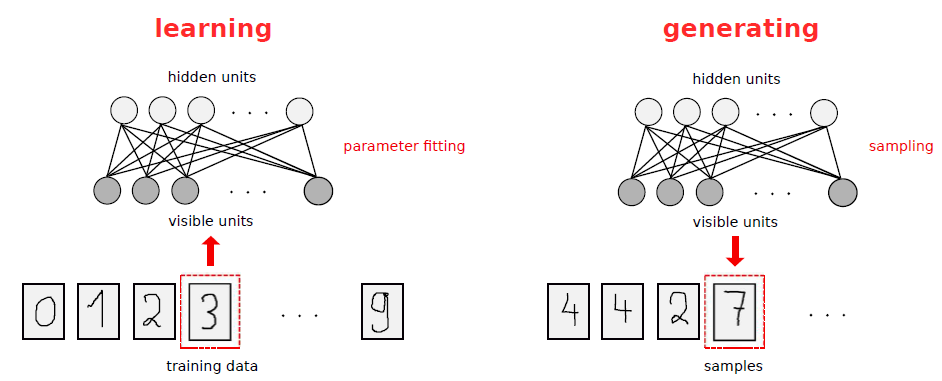
\includegraphics[width=12cm]{images/generativeRBM.png}
\captionof{figure}{Generative model of RBM. Source: A.Fischer, Ch.Igel: Training Restricted Boltzmann Machines: An Introduction. \cite{Fischer} }
\end{center}
\paragraph{Discriminative RBM}
Joint density model assumes that RBM has two sets of visible units. Besides the units representing a data vector ({\bfseries x}), there are units representing a label - {\bfseries y}. Label is therefore expressed by binary indicator variables, one of which is set to 1, indicating a particular label (for the case of handwritten images - a particular digit), while the others are set to 0. 
As a result of two sets of visible units, there are also two sets of weights: between data and hidden units ({\bfseries W}) and between label units and hidden units ({\bfseries U}). 
\begin{center}
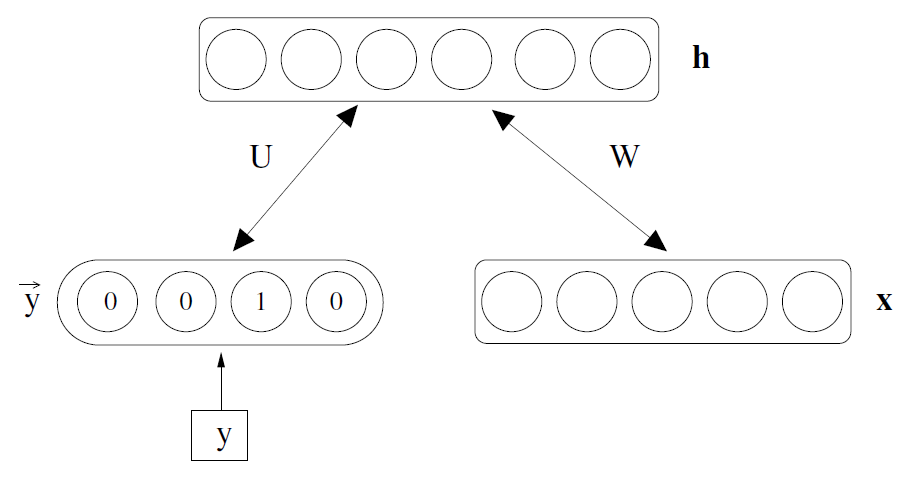
\includegraphics[width=8cm]{images/jointProbModel.png}
\captionof{figure}{Joint probability model of Restricted Boltzmann Machines. Source: \cite{Larochelle}}  
\end{center}
Model learns joint probability distribution with n-step contrastive divergence (CD) algorithm (reconstruction step is performed n-times before updating weights). Training is performed on mini-batches of the training set. In terms of the CD algorithm, it means that weights are updated after estimating a gradient on a subset of training cases (a "mini-batch"), instead of on a one single training case. Such approach is known to be more efficient, because of possible use of CPU parallelism and multi-threading.
%\begin{center}
%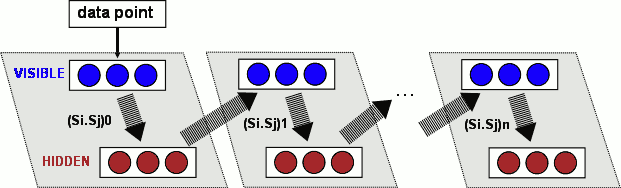
\includegraphics[width=10cm]{images/trainRBM.png}
%\captionof{figure}{Illustration of n-step contrastive divergence algorithm}  
%\end{center} 
\par Class prediction is done by choosing the most likely label given the input, under the learned model. In more detail, it fixes the visible units corresponding to the test data input and samples target units, with the use of learned weights. In the last sampling iteration the target units are set to probabilities values instead of stochastic binary units. The predicted class is the position in the binary vector with the highest probability. 
\begin{center}
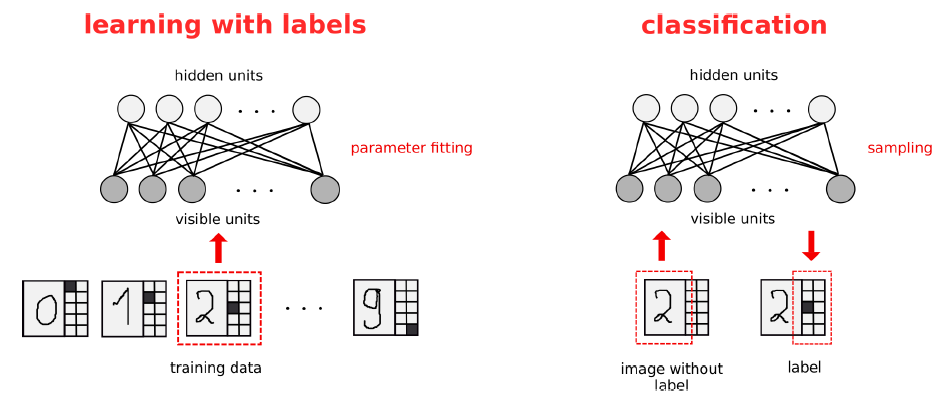
\includegraphics[width=12cm]{images/DRBM.png}
\captionof{figure}{Classification with discriminative model of RBM. Source: A.Fischer, Ch.Igel: Training Restricted Boltzmann Machines: An Introduction. \cite{Fischer} }
\end{center}
Another approach for class prediction is based on computation of free energy \cite{Hinton}. After training, a test vector is tried with each label, and the one that gives lowest free energy is chosen as the most likely class ('test-against-all-labels' prediction approach for DRBM).

\subsection{Datasets}
\par The main dataset used in the experiments was MNIST dataset of handwritten digit images. The dataset is widely used for training and testing in the field of machine learning. The images are 28 x 28 pixels, and the dataset is divided into 60,000 training cases and 10,000 test cases. The training set is further divided into a training set of 50,000 cases and a validation set of 10,000 cases. To have binary data, the pixel intensities (0-255) were scaled (0-1) and binarized with threshold of 0.5. Another possible way to make data binary is to treat the pixel intensities as probabilities and sample from the given Bernoulli distribution for each pixel. 
 
\section{Empirical Results for Discriminative RBM}
This section describes the empirical results of a RBM trained with joint density model (the third approach of using RBM's for discrimination, described by Hinton \cite{Hinton}).
\par The first aim of testing implemented RBM was finding optimal hyperparameters (optimal model parameters) The choice of optimal hyperparameters was based on the observation of reconstruction error convergence. The experiments were done on the trainset of 100 cases in 100-epoch training. 
\subsection{Monitoring progress of learning}
As it is easy to compute the squared error between the data and the reconstructions, this quantity is often a good indicator of a progress of learning \cite{Hinton}. Within experiments on Discriminative RBM, MSE was printed out after each epoch, which allowed to observe the general progress or characteristic of learning and quickly notice any abnormalities and potential problems in hyperparameter settings. 
While MSE is quite good and simple indicator of progress of learning, it is not the function that $CD_n$ is optimizing. The better indicator of what is happening during learning are graphic displays of learned filters. Plotting the weights of each unit as a gray-scale image after different numbers of epochs are shown on figures below. Filters highlight strong features in the data.
\begin{minipage}[t]{0.5\textwidth}
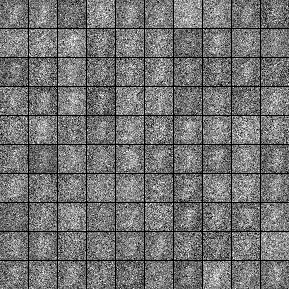
\includegraphics[width=7cm]{images/filtry_1epoch_50train.png}
\captionof{figure}{Learned filters after 1. \newline epoch of training}
\end{minipage}
\begin{minipage}[t]{0.5\textwidth}
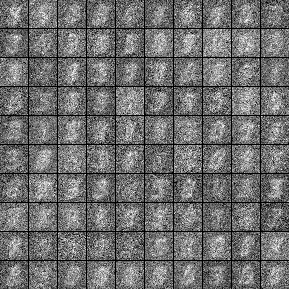
\includegraphics[width=7cm]{images/filtry_5epoch_50train.png}
\captionof{figure}{Learned filters after 5.\newline epoch of training}
\end{minipage}
\begin{minipage}[t]{0.5\textwidth}
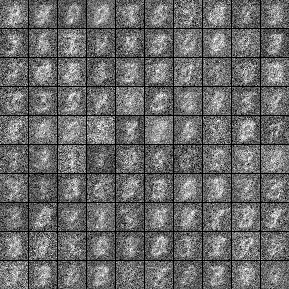
\includegraphics[width=7cm]{images/filtry_10epoch_50train.png}
\captionof{figure}{Learned filters after 10.\newline epoch of training}
\end{minipage}
\begin{minipage}[t]{0.5\textwidth}
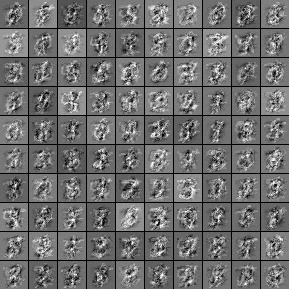
\includegraphics[width=7cm]{images/filters_epoch500_train50.png}
\captionof{figure}{Learned filters after 500.\newline epoch of training}
\end{minipage}
\subsection{The learning rate}
\par The results from training an RBM with different learning rates are shown on the figure below.
\begin{center}
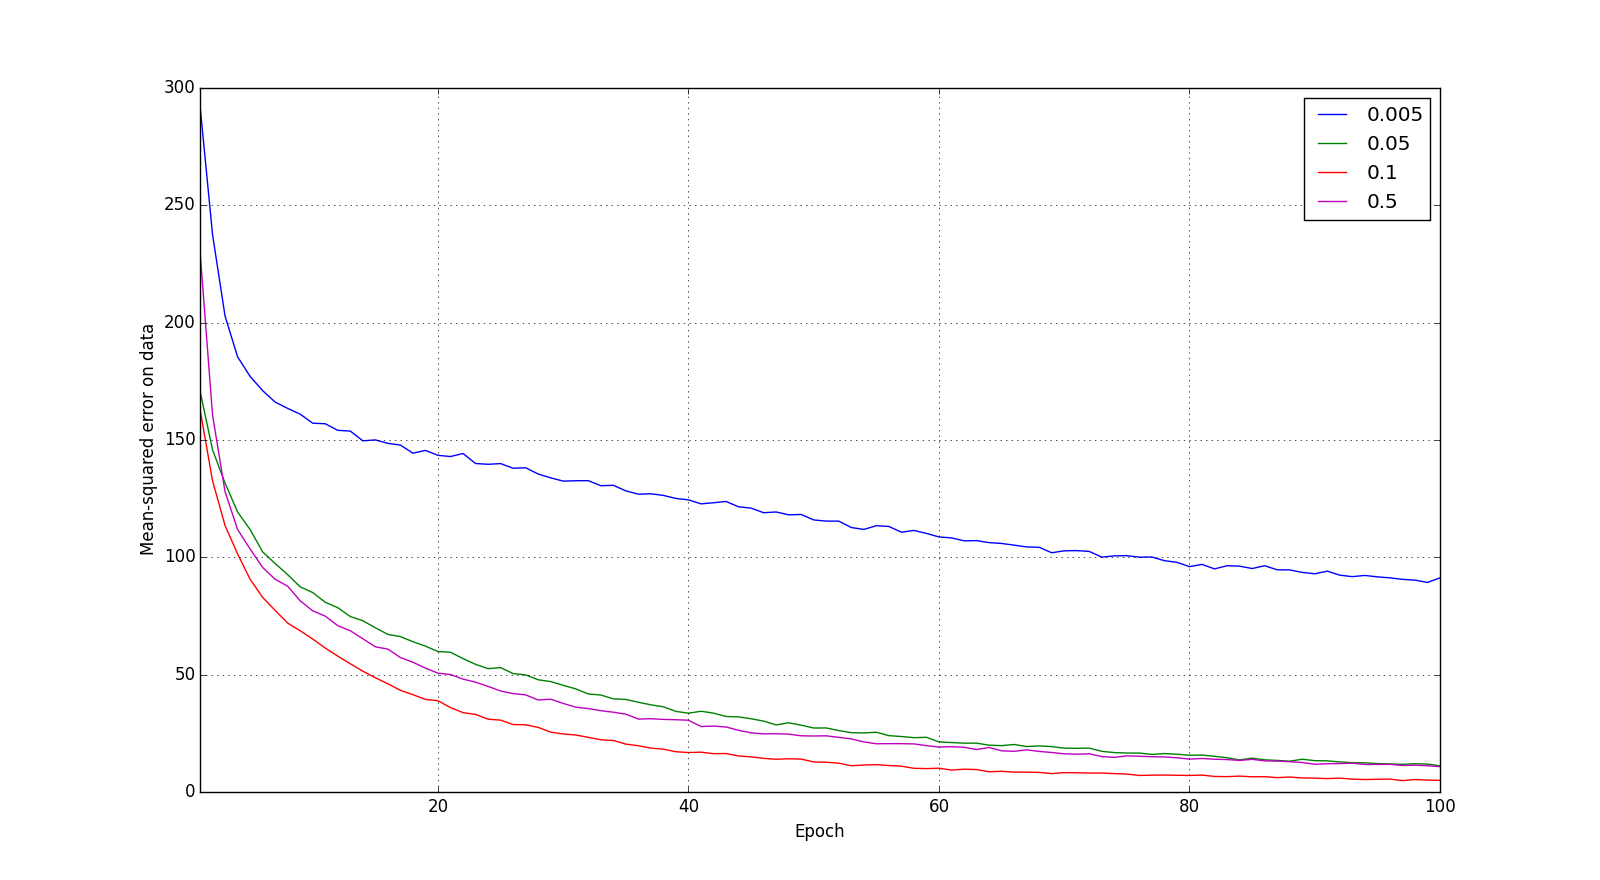
\includegraphics[width=14cm]{images/lr.png}
\captionof{figure}{Convergence comparison for different learning rates}  
\end{center}
Learning rate of a magnitude between $10^{-2}$ and $10^{-3}$ seems to be optimal. The exact optimal magnitude depends also on the training size, as tests on larger data sizes have shown (for example for smaller data sizes 0.1 was optimal, while for original sizes of 60000 - 0.01 was optimal). Additionally, too high learning rate (too high in relation to data size) caused instability and resulted in the reconstruction error increase (which is explained by Hinton \cite{Hinton} as a 'weight explosion').
\subsection{The number of hidden units}
\par The second test was done on number of hidden units. As figure below shows, the higher the number of hidden units, the better convergence of reconstruction error. On the other hand, greater hidden layer size causes longer training time (table).
\begin{center}
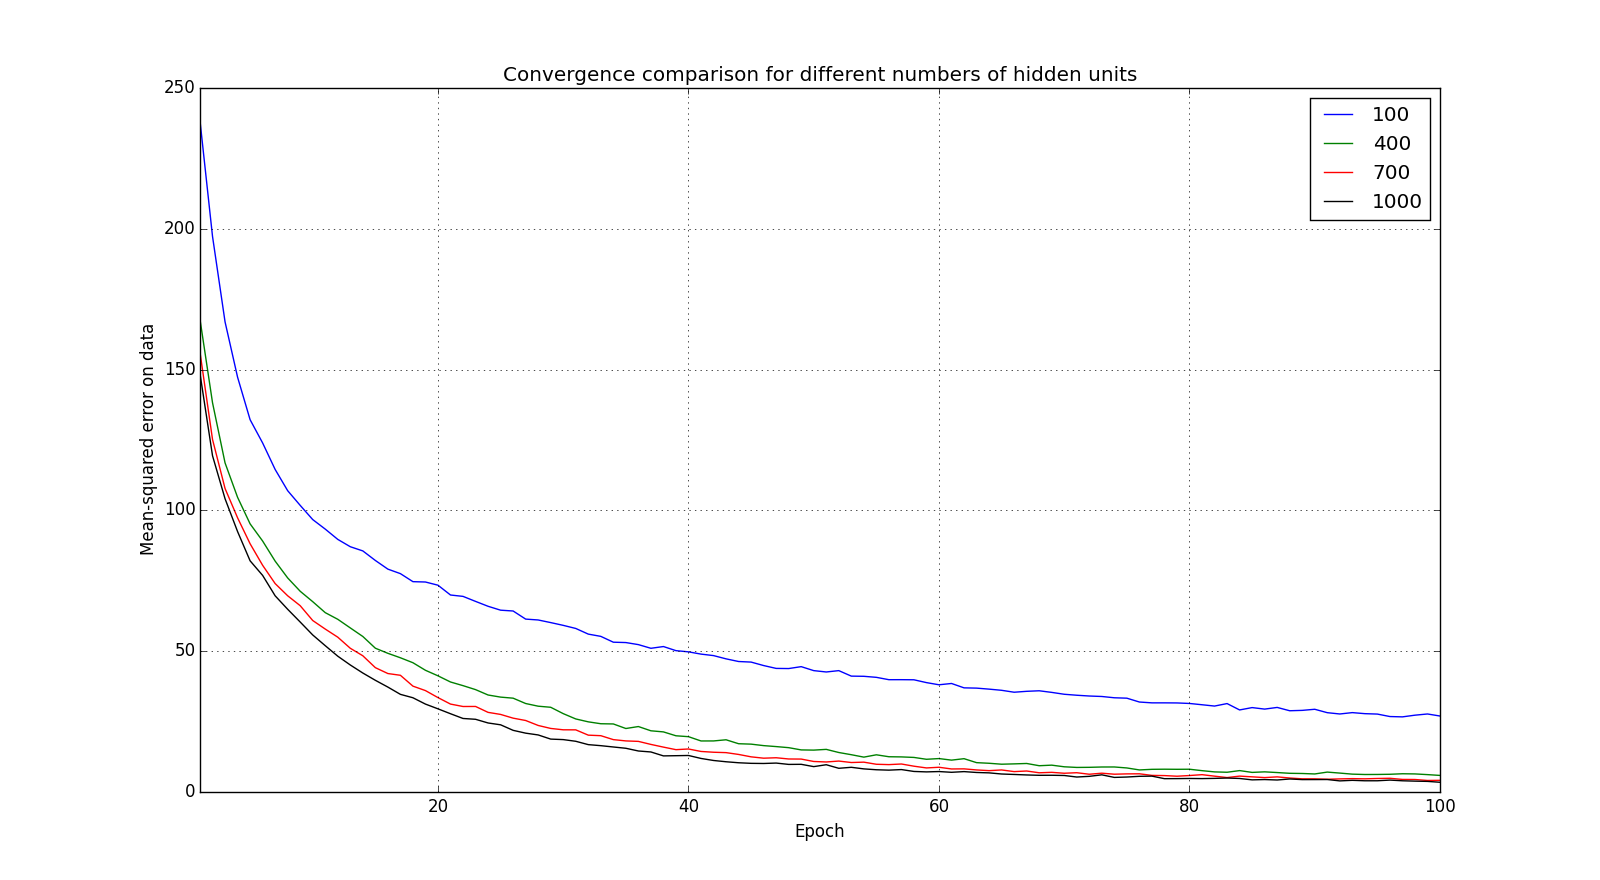
\includegraphics[width=14cm]{images/hu.png}
\captionof{figure}{Covergence comparison for different number of hidden units}  
\end{center}

\hspace{1cm}
\begin{tabular}{ | l || c | c | c | c | } 
	\hline
	Hidden units & 100 & 400 & 700 & 1000 \\ \hline
	Train time & 149.494s & 440.963s & 750.945s & 7658.844s \\ \hline
	MSE after 100 epochs & 26.981 & 5.887 & 4.149 & 3.457\\ 
	\hline 
\end{tabular}
\captionof{table}{Train time comparison for different number of hidden units. Times measured on PC Intel Pentium Dual CPU T3200 @2GHz, RAM 3 GB: CPU mean usage during test ~0.75, Memory mean usage: 2,3GB} 
\subsection{The size of a mini batch}
The mini-batch optimization procedure should use only a small number of training points for each gradient estimate: 1,5,10. Higher mini-batch sizes (such as half of training set - 50) results in relatively high reconstruction error (figure below). 
\begin{center}
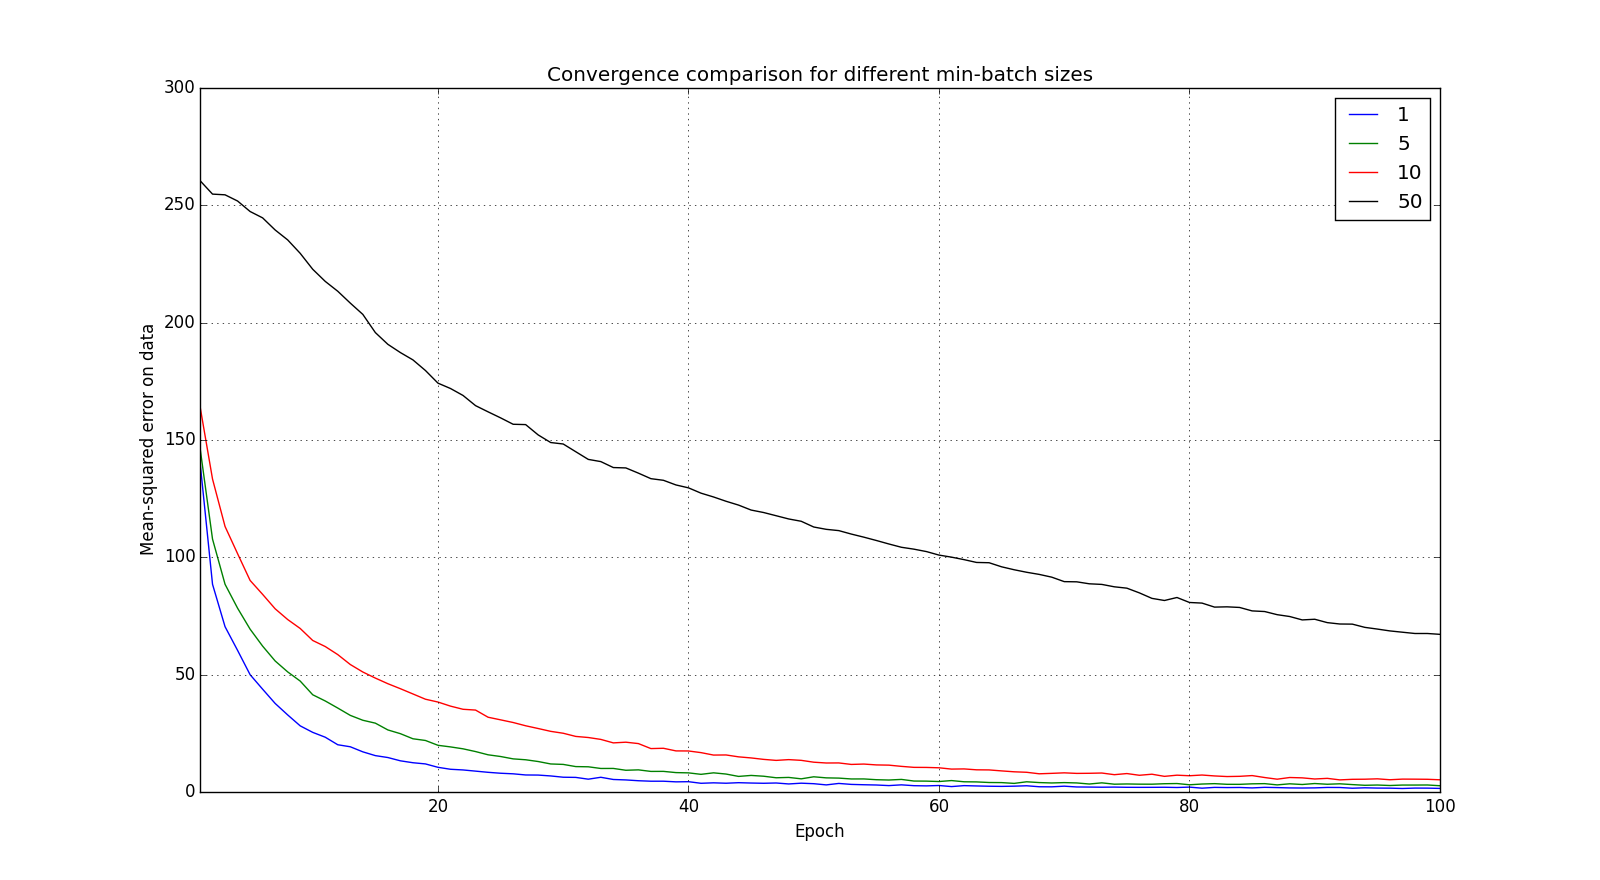
\includegraphics[width=14cm]{images/batch.png}
\captionof{figure}{Covergence comparison for different sizes of "mini-batches"}  
\end{center}
\hspace{1cm}
\begin{tabular}{|l||c|c|c|c|} \hline
Mini-batch size & 1 & 5 & 10 & 50
\\ \hline
Train time (n=100) & 1137.937s & 618.903s & 578.186s & 514.207s
\\ \hline
MSE after 100 epochs & 1.526 & 2.669 & 5.202 & 67.182
\\ \hline \end{tabular}
\captionof{table}{Train time and MSE comparison for different sizes of "mini-batch". Times measured on PC Intel Pentium Dual CPU T3200 @2GHz, RAM 3 GB: CPU mean usage during test ~0.75, Memory mean usage: 2,3GB} 
Moreover, tests on classification accuracies on 50,000 training cases and 10,000 new cases have shown that size of ten (that is equal to the number of classes) seems to be optimal (see subsection 'Classification'). The ideal case for a mini-batch would be that each sample in it would represent a different class. In other words, each mini-batch should contain one example of each class to reduce the sampling error when estimating the gradient for the whole training set from a single mini-batch \cite{Hinton}. It is possible for datasets that contain a small number of equiprobable classes. However, for the MNIST dataset, the number of samples per each class is different. Therefore it is not possible to divide the data in such a way and preserve the original size of the dataset at the same time. On the other hand MNIST dataset was already randomized, so the samples are not sorted according to the class. Randomizing a dataset along with using minibatches of size about 10 (as advised in \cite{Hinton}) seems to work optimal.
\subsection{The initial values of the weights and biases}
The weights are typically initialized to small random values chosen from a zero-mean Gaussian with a standard deviation of about 0.01. Test on initial weights with different initializations showed (see figure) that standard deviation of 0.1 features somehow better reconstruction error reduction that 0.01 and weights initialized to zeros.
Moreover starting with different generator numbers does not change the convergence significantly (compare continuous and dotted lines of the same color).
\begin{center}
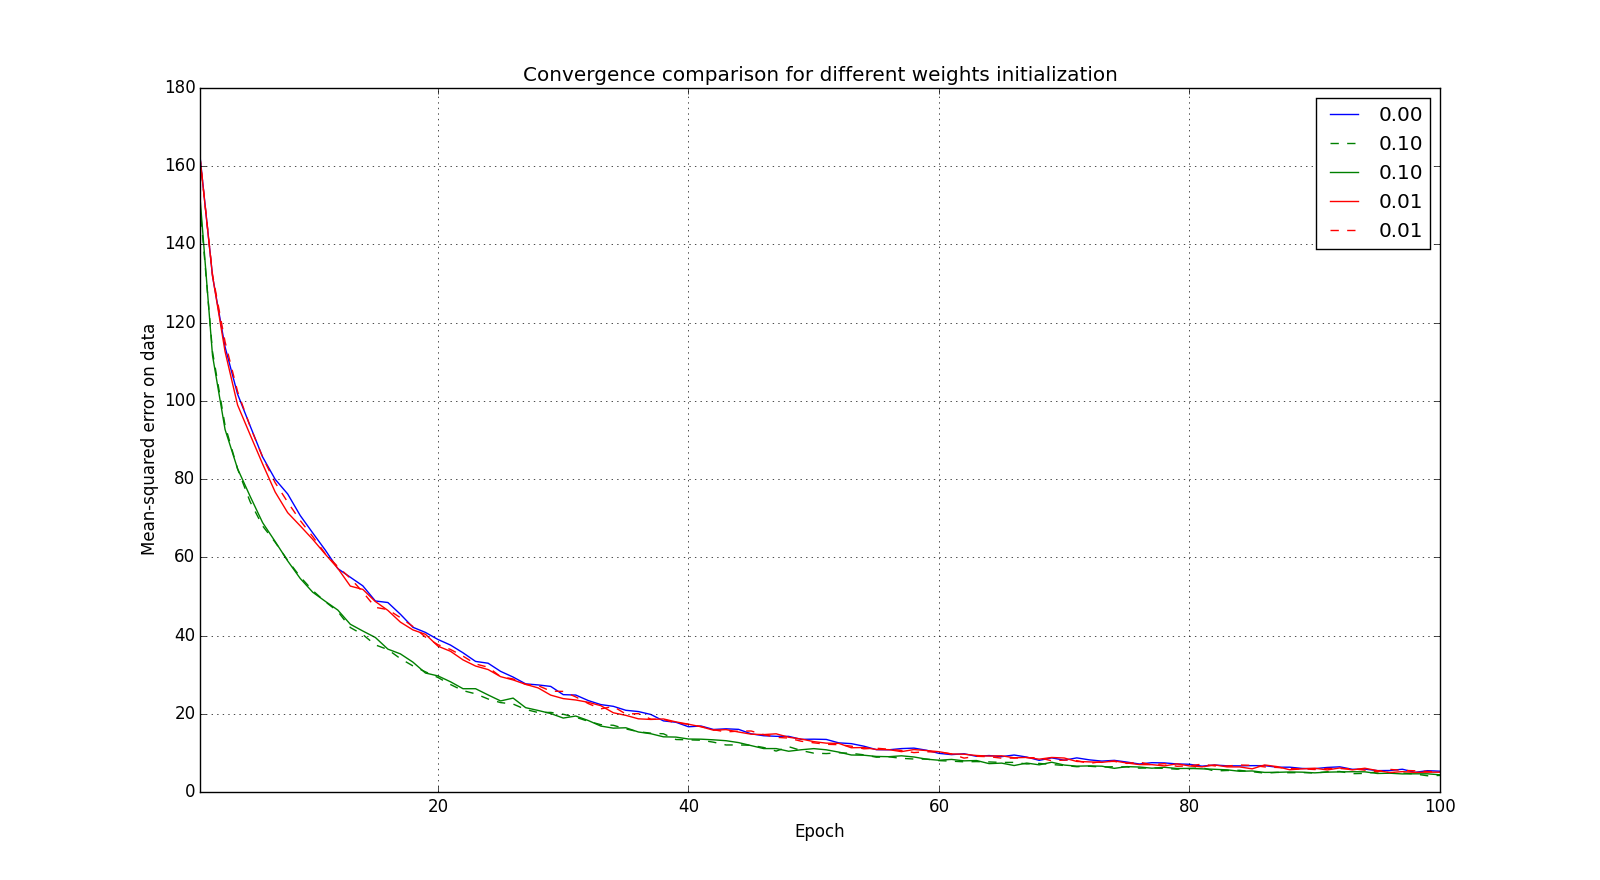
\includegraphics[width=14cm]{images/weights_seeds.png}
\captionof{figure}{Covergence comparison for different initializations of weights}  
\end{center}
\subsection{Number of steps for contrastive divergence algorithm}
All models of $CD_1$, $CD_2$ and $CD_3$ seem to be converging to the similar value, therefore, taking into account performance issues (higher number of contrastive divergence steps means longer training time - see table), it is sufficient to use one-step contrastive divergence algorithm.
\begin{center}
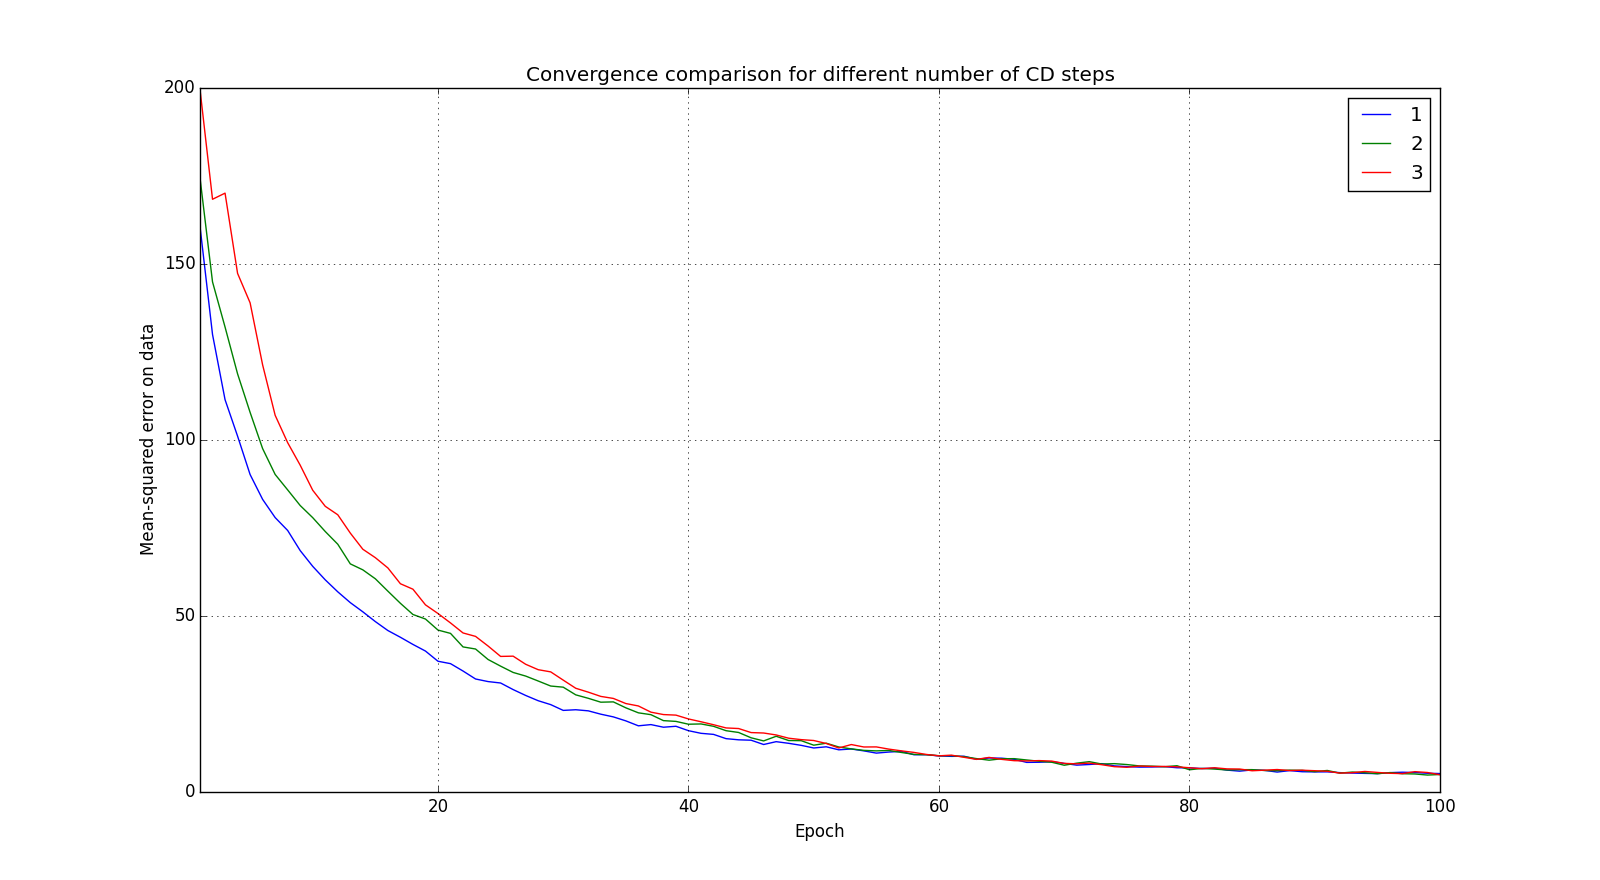
\includegraphics[width=14cm]{images/CDk.png}
\captionof{figure}{Covergence comparison for different numbers of contrastive divergence steps}  
\end{center}
\hspace{1cm}
\begin{tabular}{|l||c|c|c|} \hline
k-step CD & $CD_1$ & $CD_2$ & $CD_3$ 
\\ \hline
Train time & 529.626s & 769.475s & 959.332s 
\\ \hline
MSE after 100 epochs & 5.242 & 4.971 & 4.894 
\\ \hline \end{tabular}
\captionof{table}{Train time and MSE comparison for different numbers of contrastive divergence steps. Times measured on PC Intel Pentium Dual CPU T3200 @2GHz, RAM 3 GB: CPU mean usage during test ~0.75, Memory mean usage: 2,3GB} 
\subsection{Momentum}
Momentum is a simple method for increasing the speed of learning \cite{Hinton}. The "momentum" meta-parameter is the fraction of the previous velocity that remains after computing the gradient on a new mini-batch. The momentum method causes the parameters to move in a direction that is not the direction of steepest descent, so it could be regarded as the temporal smoothing method. It is advised (\cite{Hinton} to start with a momentum of 0.5 and once the initial progress in the reduction of the reconstruction error settles down, increase it to 0.9. 
\begin{center}
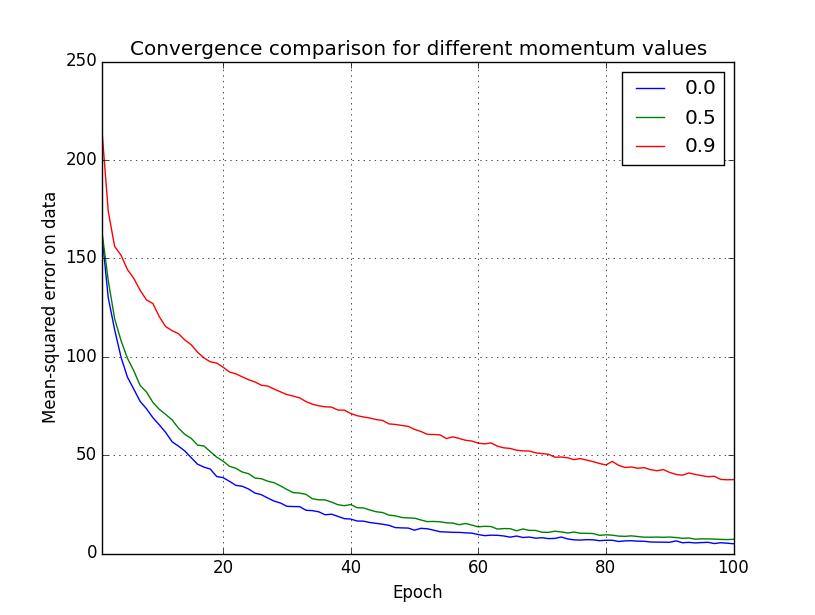
\includegraphics[width=14cm]{images/momentum.png}
\captionof{figure}{Covergence comparison for different momentum values}  
\end{center}
The basic test on three momentum values: 0, 0.5 and 0.9 showed that the best convergence and the smallest reconstruction error is reached with momentum equal to zero. It also confirms that at least at the beginning of the training it is better to lower value of momentum, and possibly increase it while reduction in reconstruction error settles down. It could also be observed that higher values of momentum caused more oscillations in learning (see figure).
\subsection{Reconstruction}
After training process and choice of an optimal model, RBM can be used to show how well it performs on the new data. Images below show a sample original image and reconstructed data. The reconstruction error after 500 epoch training falls below 1.0.
% first column
\begin{minipage}[t]{0.5\textwidth}
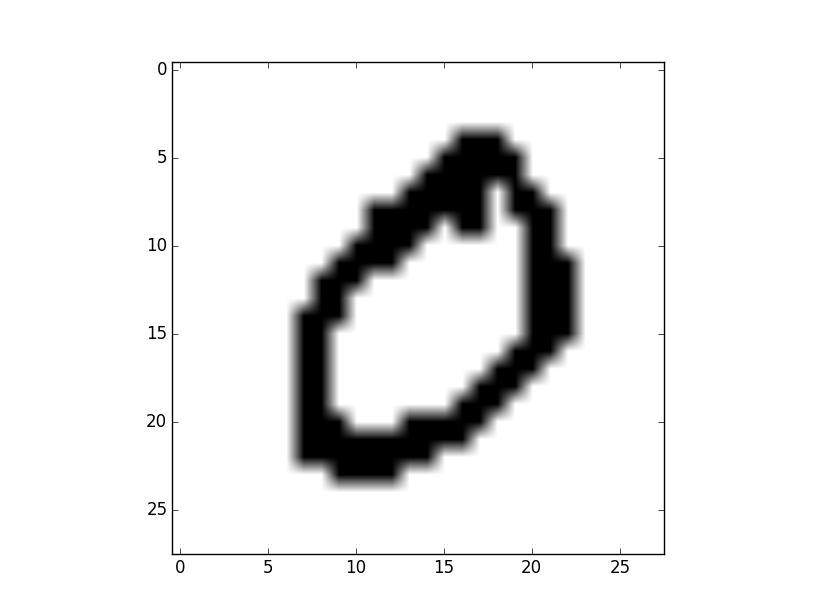
\includegraphics[width=6cm]{images/0original.png}
\captionof{figure}{Original image}
\end{minipage}
\begin{minipage}[t]{0.5\textwidth}
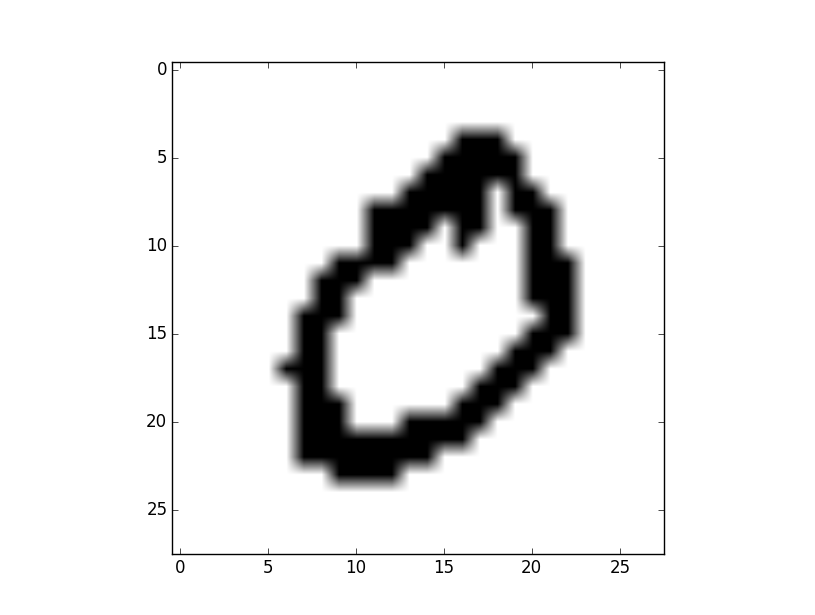
\includegraphics[width=6cm]{images/0_reconstructed_momentum00.png}
\captionof{figure}{Image reconstructed after training in 500 epochs} 
\end{minipage}
\subsection{Classification}
In the second step of experiment setup, classification metrics were computed. The most important metric for classification task is accuracy, that is, the percentage of right predictions. Accuracy was computed by comparing the label predicted by RBM classifier with the original label on test data. Wrong predictions were counted. For the preliminary results, prediction method with target units sampling was used. Table below shows classification accuracy obtained with this method on original datasets (50,000 used for training, and 10,000 new cases on which accuracy was computed). The table shows also main hyper-parameters chosen for  training the model.
\begin{center}
\hspace{1cm}
\begin{tabular}{|l||c|c|c|c|} \hline
Accuracy & Learning rate & Hidden units & Training epoch & Batch Size
\\ \hline
95,2 & 0.01 & 1000 & 100 & 10
\\ \hline
94,9 & 0.01 & 2000 & 100 & 10
\\ \hline
94,8 & 0.01 & 700 & 100 & 10
\\ \hline
94,0 & 0.01 & 700 & 100 & 50
\\ \hline
93,1 & 0.01 & 500 & 100 & 10
\\ \hline
92,7 & 0.01 & 700 & 100 & 5
\\ \hline
92,7 & 0.005 & 500 & 300 & 10
\\ \hline \end{tabular}
\captionof{table}{Classification accuracies with corresponding hyperparameters for RBM model training. Training performed on MNIST 50,000 set, classification on 10,000 new data with approach based on sampling target units.}
\end{center}
The main obstacle in testing classification accuracy with different parameters were long times of training (on personal computers training and testing on original-size MNIST dataset took days to complete one run). Yet, the models can be saved for further use.
In the second step, a prediction approach based on free energy computation was tested. Times and accuracy scores were compared with previous approach. This method proved to be incomparably faster and yielded better accuracy results. Instead of performing thousands of sampling iterations it basically computes one value (free energy) for each combination of test vector and label vector. Therefore, using free energy-based approach is much more beneficial, when the classification problem is confined to small number of classes. 
\subsection{Different types of unit - Gaussian visible units}
% Literature
\begin{thebibliography}{9}
   \bibitem[1]{Hopfield} Hopfield, J.J. (1984) \emph{Neurons with graded response have collective computational properties like those of two-state neurons} (Proc. Natl. Acad. Sci. USA)
   \bibitem[2]{Hinton} Hinton, G. (2010) \emph{A Pratical Guide to Training Restricted Boltzmann Machines.} (UTML TR 2010-003)
   \bibitem[3]{Fischer} Fischer, A., Igel, Ch. (2008) \emph{Training Restricted Boltzmann Machines: An Introduction.} 
   \bibitem[4]{Larochelle} Larochelle H., Bengio, Y. (2008) \emph {Classification using Discriminative Restricted Boltzmann Machines} (Proceedings of the 25th International Conference on Machine Learning)
\end{thebibliography}
\end{document}